\documentclass[letterpaper,12pt]{article}
\usepackage[english]{babel}
\usepackage[utf8]{inputenc}
\usepackage[nottoc]{tocbibind}
\usepackage[margin=1in]{geometry}

\usepackage[activate={true,nocompatibility},final,
			tracking=true,kerning=true,spacing=true,
			factor=1100,stretch=10,shrink=10]{microtype}

\usepackage{amsmath,apacite,graphicx,wrapfig,setspace}
\usepackage{tikz,pgfplots,algorithm,algpseudocode}
\usepackage[justification=centering]{caption}
\usetikzlibrary{matrix,arrows,calc,3d,fit}
\doublespacing

\begin{document}

\begin{titlepage}
	\begin{center}
		{\LARGE Paper Title}
	\end{center}
	% 100-200 words

\begin{abstract}

A robot control system was developed that could be taught tasks through reinforcement learning.  The system, nicknamed Fido, was designed to be universal regardless of the specific hardware inputs and outputs and does not need to be modified for the task at hand. In addition, Fido was built to learn with limited feedback, allowing humans to train Fido in a reasonable time frame. This was achieved through the training of artificial neural networks with a wire-fitted moving least squares interpolator following the $Q$-learning reinforcement algorithm and an action selection policy that utilizes a Boltzmann distribution of probability. Robots of different drive systems were simulated with sensors to test functionality, then a small robot using the Intel Edison compute module was constructed for physical testing.  The robot was successfully trained to do an array of tasks with limited feedback, such as \textbf{TASKS GO HERE}.

\end{abstract}
\end{titlepage}

\pagebreak

\section{Introduction}

The most prevalent control system used in mobile robotics is a procedurally programmed expert system (Biggs \& MacDonald, 2003).  Such systems use conditional logic in order to emulate a desired behavior.  However, such systems are limited in numerous respects.  First, they can only perform the specific task for which they were programmed to accomplish; the entire software must be rewritten in order to change the target task.  Second, they rely on a knowledge of the inputs and outputs to the robot (such as sensors and motor control) in order to function.  The purpose of Fido was to solve both of these problems, allowing a universal general control system for robots that can be assigned tasks ``in the field'' using reinforcement learning.  

We chose to approach this problem with artificial neural networks; function appropriators modeled after nature with the capability to take in a large number of inputs to produce an output.  Neural networks are commonly used to solve tasks that are challenging using traditional rule-based programming, making them perfect for our task.  The control system was named Fido for the name's connotations to training an intelligent organism. 

\section{Neural Network Background}

\subsection{Artificial Neuron Introduction}

% figure of a bio neuron

The human brain is composed of billions of neurons: interconnected electrically excitable cells that form the basis of our intelligence.  Each neuron has synapses that receive electrical signals from multiple other neurons.  If the sum of these inputs is greater than a certain value, the neuron fires, generating a voltage at its axon.  The axon, or the output of the neuron cell, is itself connected to a synapse of another neuron.  The interconnections of these neurons form a massive network, where a huge number of inputs are processed in parallel to a set of outputs.  The basis of artificial neural networks is to simulate the mathematical properties of these neurons in order to perform similar tasks of mass parallel computation.

\begin{figure}[ht]
	\centering
	\def\layersep{2.5cm}
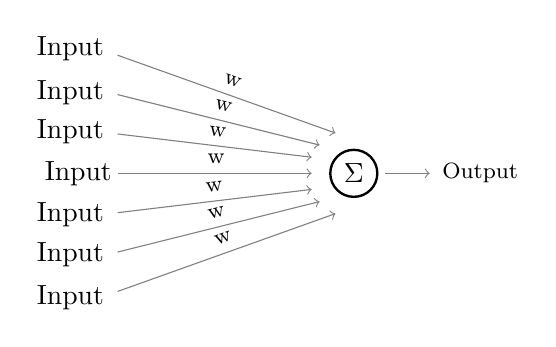
\begin{tikzpicture}[shorten >=1pt,->,draw=black!50, node distance=\layersep]
    \tikzstyle{every pin edge}=[<-,shorten <=1pt]
    \tikzstyle{neuron}=[circle,line width=0.3mm,draw=black,minimum size=17pt,inner sep=0pt]
    \tikzstyle{annot} = [text width=4em, text centered]


    \draw[->] (-3,1.5) -- (-.2,.5) node[sloped,midway,above] {\footnotesize w} node[left=3.4cm,above=.8cm]{Input};
    \draw[->] (-3,1) -- (-.4,.35) node[sloped,midway,above] {\footnotesize w} node[left=3.2cm,above=.4cm]{Input};
    \draw[->] (-3,0.5) -- (-.5,.2) node[sloped,midway,above] {\footnotesize w} node[left=3.1cm,above=.05cm]{Input};
    \draw[->] (-3,0) -- (-.5,0) node[sloped,midway,above] {\footnotesize w} node[left=2.45cm]{Input};
    \draw[->] (-3,-0.5) -- (-.5,-.2) node[sloped,midway,above] {\footnotesize w} node[left=3.1cm,below=.05cm]{Input};
    \draw[->] (-3,-1) -- (-.4,-.35) node[sloped,midway,above] {\footnotesize w} node[left=3.2cm,below=.4cm]{Input};
    \draw[->] (-3,-1.5) -- (-.2,-.5) node[sloped,midway,above] {\footnotesize w} node[left=3.4cm,below=.8cm]{Input};
    
    \node[neuron] (0,0) {$\Sigma$};

    \draw[->] (.4,0) -- (1,0) node[right] {\footnotesize Output};
\end{tikzpicture}
	\caption{Single Neuron Diagram}
\end{figure}

An artificial neuron simply a mathematical model of a biological neuron, and therefore its functionality is very similar.  Each neuron has multiple inputs, each with an individual weight, and one output.  The weight of an input is simply a positive or negative fraction that govern the impact of each input on the single output.  An artificial neuron's set of weights determines its function, and the function of each neuron in a neural network (in addition to the arrangement of the network) determines the function of the network as a whole.  This will become important as we discuss training Fido's neural network, however for the moment we will adjust our focus to the output of an artificial neural network.  By summing each input multiplied by its individual weight we reach a value called the activation, expressed as such mathematically for each input $x$ and weight $w$:

\begin{equation}
	a=\sum_{i=0}^{i=n}x_i w_i
	\,.
\end{equation}

If this activation value is less than a certain threshold, the output is zero.  If it is greater than the threshold, the output is one.  This activation function most closely resembles the biological model of a neuron, a binary step function.  However, a binary output can be somewhat limiting for many applications of neural networks.  For example, many of Fido's outputs are gradient rather than linear; as an example, an LED can be given a brightness.  For this purpose alternate activation functions can be used with gradient outputs.  One such function is a sigmoid function, expressed as such:

\begin{equation}
	O(a) = \cfrac{1}{1+e^{-\frac{a}{p}}}
	\,,
\end{equation}

\noindent for each output $O$, activation $a$, and constant $p$.  The sigmoid activation function can also be graphed as below.

\begin{figure}[ht]
	\centering
	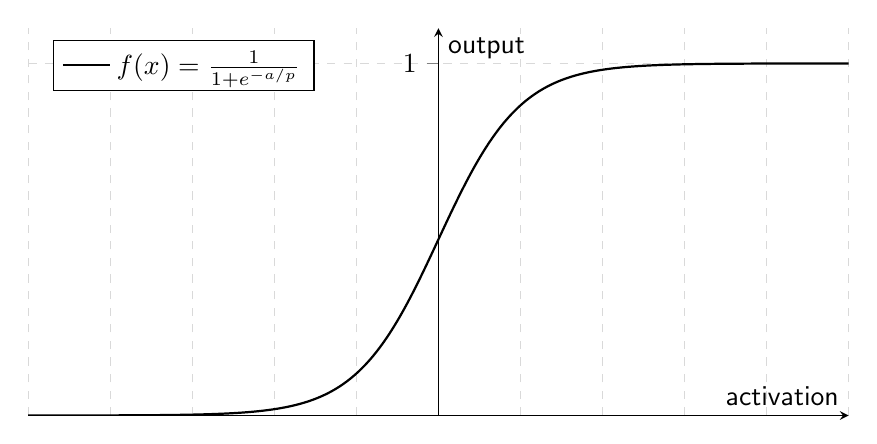
\begin{tikzpicture}[font=\sffamily]
    \begin{axis}[
    	legend pos=north west,
        axis x line=middle,
        axis y line=middle,
        grid = major,
        width=12cm,
        height=6.5cm,
        grid style={dashed, gray!30},
        xmin=-1,xmax= 1,ymin= 0,ymax= 1.1,
        xlabel=activation,ylabel=output,
        tick align=outside,
        ytick={1},
        xmajorticks=false,
        enlargelimits=false]
      \addplot[domain=-1:1,black,thick,samples=500] {1/(1+exp(-10*x))}; 
      \addlegendentry{$f(x)=\frac{1}{1+e^{-a/p}}$}
    \end{axis} 
\end{tikzpicture}
	\caption{Sigmoid Function Graph}
\end{figure}

This provides us with a gradient output, however output is still limited to positive values.  An alternative activation function which allows outputs ranging from -1 to +1 is the hyperbolic tangent activation function:

\begin{equation}
	O(a) = \tanh(a)% = \cfrac{e^a-e^{-a}}{e^a+e^{-a}}
	\,.
\end{equation}

The hyperbolic tangent activation can be graphed as such, demonstrating its greater range and gradient output.

\begin{figure}[ht]
	\centering
	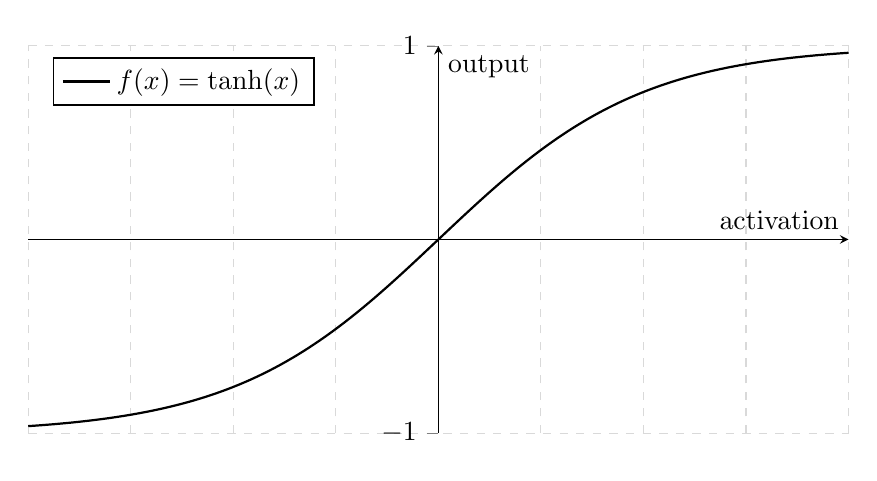
\begin{tikzpicture}
    \begin{axis}[
    	legend pos=north west,
        axis x line=middle,
        axis y line=middle,
        grid = major,
        width=12cm,
        height=6.5cm,
        grid style={dashed, gray!30},
        xmin=-2,xmax= 2,ymin= -1,ymax= 1,
        xlabel=activation,ylabel=output,
        tick align=outside,
        ytick={-1,1},
        xmajorticks=false,
        enlargelimits=false]
      \addplot[domain=-2:2,black,thick,samples=500] {tanh(x)}; 
      \addlegendentry{$f(x)=\tanh(x)$}
    \end{axis} 
\end{tikzpicture}
	\caption{Hyperbolic Tangent Function Graph}
\end{figure}

\subsection{Feedforward Neural Network}

A traditional method of arranging artificial neurons in a neural network is called a feedforward network.  Neurons are connected as previously described: the output of each neuron is connected to one of the inputs of another neuron.  These neurons are organized into layers, as described in the following figure: % ogres have layers

\begin{figure}[ht]
	\centering
	\def\layersep{2.5cm}
\begin{tikzpicture}[shorten >=1pt,->,draw=black!50, node distance=\layersep,font=\sffamily]
    \tikzstyle{every pin edge}=[<-,shorten <=1pt]
    \tikzstyle{neuron}=[circle,line width=0.3mm,draw=black,minimum size=17pt,inner sep=0pt]
    \tikzstyle{annot} = [text width=4em, text centered]

    \foreach \name / \y in {1,...,4}
        \node[neuron, pin=left:Input \y] (I-\name) at (0,-\y) {};

    \foreach \name / \y in {1,...,5}
        \path[yshift=0.5cm]
            node[neuron] (H-\name) at (\layersep,-\y cm) {};

    \node[neuron,pin={[pin edge={->}]right:Output}, right of=H-3] (O) {};

    \foreach \source in {1,...,4}
        \foreach \dest in {1,...,5}
            \path (I-\source) edge (H-\dest);

    \foreach \source in {1,...,5}
        \path (H-\source) edge (O);

    %\draw[->] (5,-2.9) -- (5,-5) -- (1,-5) -- (1,-4.5);
    %\node (1,-4.5) {Error back propagation}

    \node[annot,above of=H-1, node distance=1cm] (hl) {Hidden layer};
    \node[annot,left of=hl] {Input layer};
    \node[annot,right of=hl] {Output layer};
\end{tikzpicture}
	\caption{Single Output Feedforward Network}
\end{figure}

Initial inputs are first sent into the input layer.  Next, the output of each input layer neuron is sent into each neuron in the hidden layer.  The hidden layer processes the inputs to outputs using an activation function and a weight value for each input.  There can be any number of hidden layers in a neural network, depending on the complexity of the computation being performed.  Finally the outputs from the last hidden layer neurons are sent into each neuron of the output layer, where the final outputs are processed.  A concrete example of a feedforward network is that of Fido.  Sensor inputs such as light and sound are sent into the input layer.  After the signals have passed through to the output layer, the outputs from the output layer are sent to outputs such as motors, LEDs, and buzzers.   The purpose of training a neural network is to make input values correspond to the correct output values, depending on the desired behavior.  An example could be making Fido drive when light is applied.  The way to give a neural network desired behavior is by controlling the weights of each neuron using a learning algorithm.

\section{Learning Implementation}

% Intro text here; a sentence or two
Intro text.

\subsection{Q-Learning}

Reinforcement learning seeks to find the optimal action to be undertaken for a given state through trial and error. In the context of Fido, an action could be the playing of a note or driving straight forward, while the state could the amount of light detected by the robot or how near the robot is to another object. Once an action is performed, a reward and a new state are given back to the reinforcement learning algorithm.  As actions are performed over time a reinforcement learning algorithm sharpens its ability to receive reward.

$Q$-Learning \cite{watkins} is a popular reinforcement learning algorithm that works by learning an action-value function $Q$ that takes an state-action pair as an input and outputs an expected utility value of performing that action in that state. This utility value is know as the $Q$-value. The $Q$-value is a combination of immediate reward and expected future reward. Every reward iteration, the $Q$-value of an state-action pair is updated as such:

\begin{equation}
	Q(s, a) := Q(s, a)(1 - \alpha) + \alpha(R + \gamma \max Q(s_{t+1}, a))
	\,,
\end{equation}

Where $a$ is the action carried out, $s$ is the initial state, $R$ is the reward received, and $s_{t+1}$ is the new state. $\alpha$ is the learning rate of the algorithm. The learning rate determines the rate of convergence by diminishing or amplifying the changes made to the $Q$-value each reward iteration. $\gamma$ is the devaluation factor, which determines the weight given to future rewards. A devaluation factor approaching $\gamma=0$ will force the algorithm to only value immediate reward, while a devaluation factor approaching $\gamma=1$ will make it focused on high long term reward.

The $Q$-Learning algorithm had to be immediately modified in two ways to make it suitable for Fido. Its scalability had to be improved, and it had to be able to work in continuous state-action spaces. 

$Q$-learning in its simplest form uses a table to model the $Q$ function, storing past state-action pairs and each pair's respective $Q$-value.  However, this strategy lacks scalability. In large state-action spaces, such as those Fido will have to perform in, the amount of data and computation needed to maintain such a table renders such a strategy impractical. Since Fido will be working in large state-action space, it is necessary to use a function approximator to model $Q$. A feedforward neural networks were chosen for this task for their ability to model non-linear functions, lightweight computational footprint, high trainablility.

Conventional $Q$-Learning is discrete. No relation is made between states or actions, and every action for each state must be performed individually repeatedly in a noisy feedback system to determine its $Q$-value. However, Fido will work in a large, continuous state-action spaces where relations made between (state-action, $Q$-value) pairs can drastically reduce the number of reward iterations needed for convergence. An example of a task that would benefit from continuity is teaching Fido to adjust the speed of its motors based on the intensity of light that the robot detects. There is an obvious gradient relation between the (state-action, $Q$-value) pairs in this task and with a limited number of $Q$-values known, it is possible to correctly model $Q$.

\subsection{Wire-Fitted Q-Learning}

To accommodate continuous action-spaces, we coupled a wire-fitted moving least squares interpolator with our feedforward neural network as described in \cite{wirefit}. 

Feed-forward neural networks can generalize between states in $Q$-Learning problems with discrete actions as described in \cite{rummery}. To extend this implementation to a continuous action space, our feed-forward neural network outputs discrete ``wires'' when given a state. Each wire consists of an action with its respective $Q$-value for the state given to the neural network. These wires may be interpolated to model $Q$, allowing us to get the $Q$-value of any action performed in state given as an input to the network. The interpolator used in Fido is a wire-fitted moving least squares interpolator used in the context of a memory-based learning system in \cite{baird}.

The wire-fitting function calculates $Q$-value of an action $\hat{a}$ for a state $s$ given a set of $n$ actions $a$ each with a respective $Q$-value $q$ as such:

\begin{equation}
	Q(a, s) = \frac{\sum_{i=0}^{n}\frac{q_i}{||\hat{a}-a_i||^2+c(q_{max}-q_i)+k}}{\sum_{i=0}^{n}\frac{1}{||\hat{a}-a_i||^2+c(q_{max}-q_i)+k}}
	\,,
\end{equation}

where $q_{max}$ is the greatest $Q$-value among the set of $Q$-values $q$, and $k$ is a small constant that avoids division by 0. $c$ is the smoothing factor. The greater the smoothing factor, the smoother the interpolated function.


\ref{fig::wirefitexample} is an example of interpolation on a set of wires. The graph shows the value of one-dimensional actions plotted against their respective $Q$-value.

\begin{figure}[ht]
    \centering
    \includegraphics[height=5cm]{Figures/WireFit.png}
	\caption{Moving Least Squares Interpolator (adapted from Gaskett, Wettergreen, \& Zelinsky, 1999)}
    \label{fig::wirefitexample}
\end{figure}

The wire-fitting function has many properties that make it especially suited for Fido.

Updates to the $Q$-value and oftentimes choosing which action to perform require that $Q$-max is computed. As proved in \cite{baird}, the maximum $Q$-value outputted by the wire-fitting function is the maximum $Q$-value out of the set of wires that the function takes as an input. This makes it extremely computationally cheap to 

\section{Simulation}

The robot model chosen for simulation was modeled after easily producible robots on the same scale.  The software driving the simulation was intended to be portable enough to work on a hardware implementation, and the model facilitates this goal as well.  Additionally, the robot model would have to be easily trainable and debuggable when implemented in hardware; as such, the use of a Geiger counter as an input would be unfavorable.  Lastly the sensors and design chosen had to facilitate the concept of natural learning, modeling after nature to some degree.

\subsection{Robot Inputs and Outputs}

Multiple inputs were modeled for simulation with outlets for control both by a human operator using sliders and by programmed handlers using a bridge class.  A microphone and light sensor were chosen as clear, human modifiable inputs that model after nature and could easily be used for reinforcement training.  An infrared light sensor was added as another easily controller variable in a testing setup: a human operator could easily bring closer and farther an IR LED for purposes of training.   Additionally sensors for battery level, three axes of accelerometers, and three axes of gyroscopes were added as more complex inputs for Fido to master.  The last sensor added was a three axis radio receiver.  The purpose of the receiver was to allow location based training of the robot relative to a radio beacon, such as following the beacon or avoiding it.  The radio sensor is a stand-in for Bluetooth, Wi-Fi, or any other radio technology; it is common practice in many areas of robotics to use radio beacons for localization.

\begin{figure}
	\centering
	\fbox{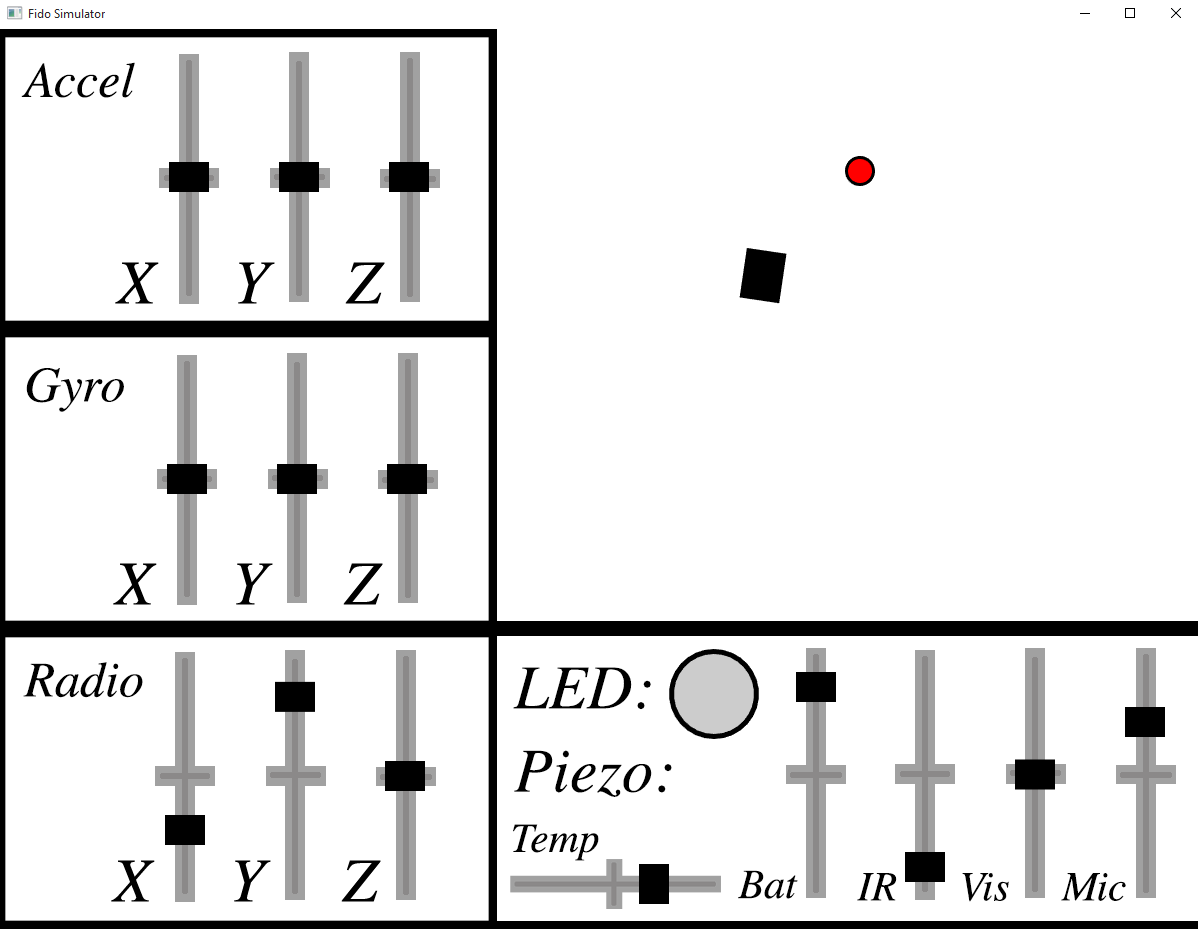
\includegraphics[height=10cm]{Figures/Screenshot.png}}
	\caption{Screenshot of the Fido Simulator Graphical User Interface}
\end{figure}

Fido's outputs were chosen similarly.  Two motors allow a drive mechanism known as differential drive, which will be discussed further in the following section.  A buzzer of varying tone and frequency and a multicolor LED complete the set of outputs.  

\subsection{Implementation and Kinematics}

A graphical user interface was implemented using the SFML multimedia library for C++.  Sliders manually adjust inputs such as accelerometer and gyroscope sensor axes, battery life, and temperature.  A colored circle displays the output of the multicolor LED, while the frequency and volume of the piezoelectric speaker are displayed on the bottom bar.   Initially vectors of motor values were displayed graphically in the top right of the window.  This made sense for initial testing purposes: both competition entrants were experienced with differential drive robots, and could easily visualize robot movement from robot vectors.  However, as we decided to do more development on the simulator we wanted to allow more complex training on the simulator, such as path following.  Such training requires a visual kinematic simulation of the robot model.

\begin{figure}[ht]
	\centering
	\begin{tikzpicture}
	\begin{scope}[rotate=-20]
		\tikzset{dot/.style={circle,fill=#1,inner sep=0,minimum size=.5pt}}

		\draw[ultra thin] (0,0) -- (8,0);
		\draw[pattern=north west lines,thick](3,0) ellipse (0.4cm and 1.4cm);
		\draw[pattern=north west lines,thick](7,0) ellipse (0.4cm and 1.4cm);

		\node[circle,fill,inner sep=-2pt,label=below:${(x,y)}$] at (5,0){};
		\node[circle,fill,inner sep=-2pt,label={[xshift=.6cm, yshift=0.1cm]$\theta$}] at (0,0){};
		\node[circle,fill,inner sep=-2pt,label={[xshift=.2cm, yshift=-1.5cm]$\omega$}] at (0,0){};
		\node at (0,-.4) {ICC};

		\draw[->] (.5,0) arc (0:110:.5cm);
		\draw[->] (1,0) arc (0:-110:1cm);
		
		\draw[->] (2.3,-1) -- (2.3,1.5);
		\node at (1.8,.8) {$V_{left}$};
		\draw[->] (7.7,-1) -- (7.7,1.5);
		\node at (8.3,.8) {$V_{right}$};

		\draw[<->] (0,-2) -- (5,-2);
		\node at (2.5,-2.3) {$R$};

		\draw[<->] (3,2) -- (7,2);
		\node at (5,2.3) {$l$};
	\end{scope}
	
	\draw[step=.5cm,gray,ultra thin] (-1,1.5) grid (9,-4.5);
\end{tikzpicture}
	\caption{Differential Drive Kinematics Diagram}
\end{figure}

Fido's two motors are arranged in a differential drive arrangement.  Driving the left motor acts as a force vector on the left side of the robot, creating a torque around the right wheel.  The same applies with the right wheel.  When both motors are activated together, the motor drives straight.  Each motor has a value ranging from -100 to 100, where -100 is full power backwards, 0 is stopped, and 100 is full power forwards.   In order to render robot movement in the simulator, we must first model the movement that our robot will take.

Every movement the robot takes can be interpreted as a rotation of radius $R$ around the ICC, or instantaneous center of curvature.   If the robot is moving straight, this radius is simply infinite.   The robot travels at an angular velocity $\omega$ around the circle, and at any given moment is at the coordinates $(x,y)$ and orientation $\theta$.  The length of the robot from wheel-center to wheel-center is defined as $l$, while the velocity vectors of each motor are defined as $V_l$ and $V_r$ respectively.  The passing of time from the last call of motor values is defined as $\Delta t$.  We can solve for $R$ and $\omega$ at any point using the following equations:
\begin{align*}
	R &= \cfrac{l}{2} \times \cfrac{V_l + V_r}{V_r - V_l}\\
	\omega &= \cfrac{V_r - V_l}{l}
\end{align*}

Using these values we can easily define the ICC as $(x - R\sin\theta,y + R\cos\theta)$.  We then solve for the robot's new position, defined as coordinates $(x',y')$ and orientation $\theta'$.

\begin{equation}
	\begin{bmatrix}
	    x'      \\
	    y'      \\
	    \theta' \\
	\end{bmatrix} =
	\begin{bmatrix}
		\cos(\omega\Delta t) & -\sin(\omega\Delta t) & 0 \\
		\sin(\omega\Delta t) & \cos(\omega\Delta t)  & 0 \\
		0                    &                       & 1 \\
	\end{bmatrix}
	\begin{bmatrix}
		x - ICC_x  \\
		y - ICC_y  \\
		\theta     \\
	\end{bmatrix} + 
	\begin{bmatrix}
		ICC_x          \\
		ICC_y          \\
		\omega\Delta t \\
	\end{bmatrix}
\end{equation}

A brief inspection of these equations verify their performance in certain use cases.  If $V_r = -V_l$ $R$ becomes zero, as the robot turns around it's center.  If $V_r = V_l$ $R$ becomes infinite, as the robot is traveling in a straight line.  Using these equations we were were able to fully simulate Fido's kinematic model, and attach simulator motor inputs to Fido's outputs to visualize learning taking place.   

The black rectangle in the upper right corner of the simulator is the robot, having been moved as part of training.  The red dot near the rectangle is a graphical representation of a radio beacon.  As adjusting sliders to represent the location of a radio beacon relative to the robot would be impractical, we decided to implement a beacon that could be placed and dragged by right clicking on the simulator.  Simulated sensor readings of beacon strength on two axis are gathered using an inverse square law, as applies to radio waves in general.  These readings are then displayed in the sliders and can be manually altered as well.  The radio beacon can be removed by a human operator by pressing the ``p'' key.  This was especially helpful in the task of training Fido to follow a radio beacon.


\section{Results}

Results, testing, and applications go here.

\subsection{Training Methods}

\subsection{Findings}

\subsection{Further Applications}

\section{Discussion}

\subsection{Future Software Research}

Currently, the number of wires that our neural network outputs is constant. However, the complexity of the functions that the wire-fitting function has to model varies from task to task. To add to the portability of Fido, we plan on implementing a method of dynamically changing the number of wires that the neural network outputs. Such a method would gage the variance and bias that the interpolator is experiencing. Variance is the deviation of a function from its mean. Bias is the error that results from under fitting. The wire-fitting function's variance could be measured in a range of actions. Bias could be measured as the moving average of the wire-fitted interpolator function's error at predicting Q-values, or the moving average of the distance that the wire-fitting function's wires have to move during gradient descent. Our proposed method would look to reduce $bias^2 + variance$ by increasing the number of wires if there is high bias squared and decreasing the number of wires if there is high variance. Each time a wire is removed or added to create a new set of wires, this set of wires will be changed to best model the wire-fitting function formed by the past set of wires.

The topology of our feed-forward neural networks is static throughout Fido's lifetime. To increase the generality of Fido, we would like to research ways to evolve the topology of Fido's neural network as performs action and receives reward. This may mean measuring variance and bias values and determining the direction of $bias^2 + variance$ as outlined above, but may also take the form of an existing variation of back propagation, of which there are many.

\subsection{Hardware Implementation}

\begin{figure}[ht]
	\centering
	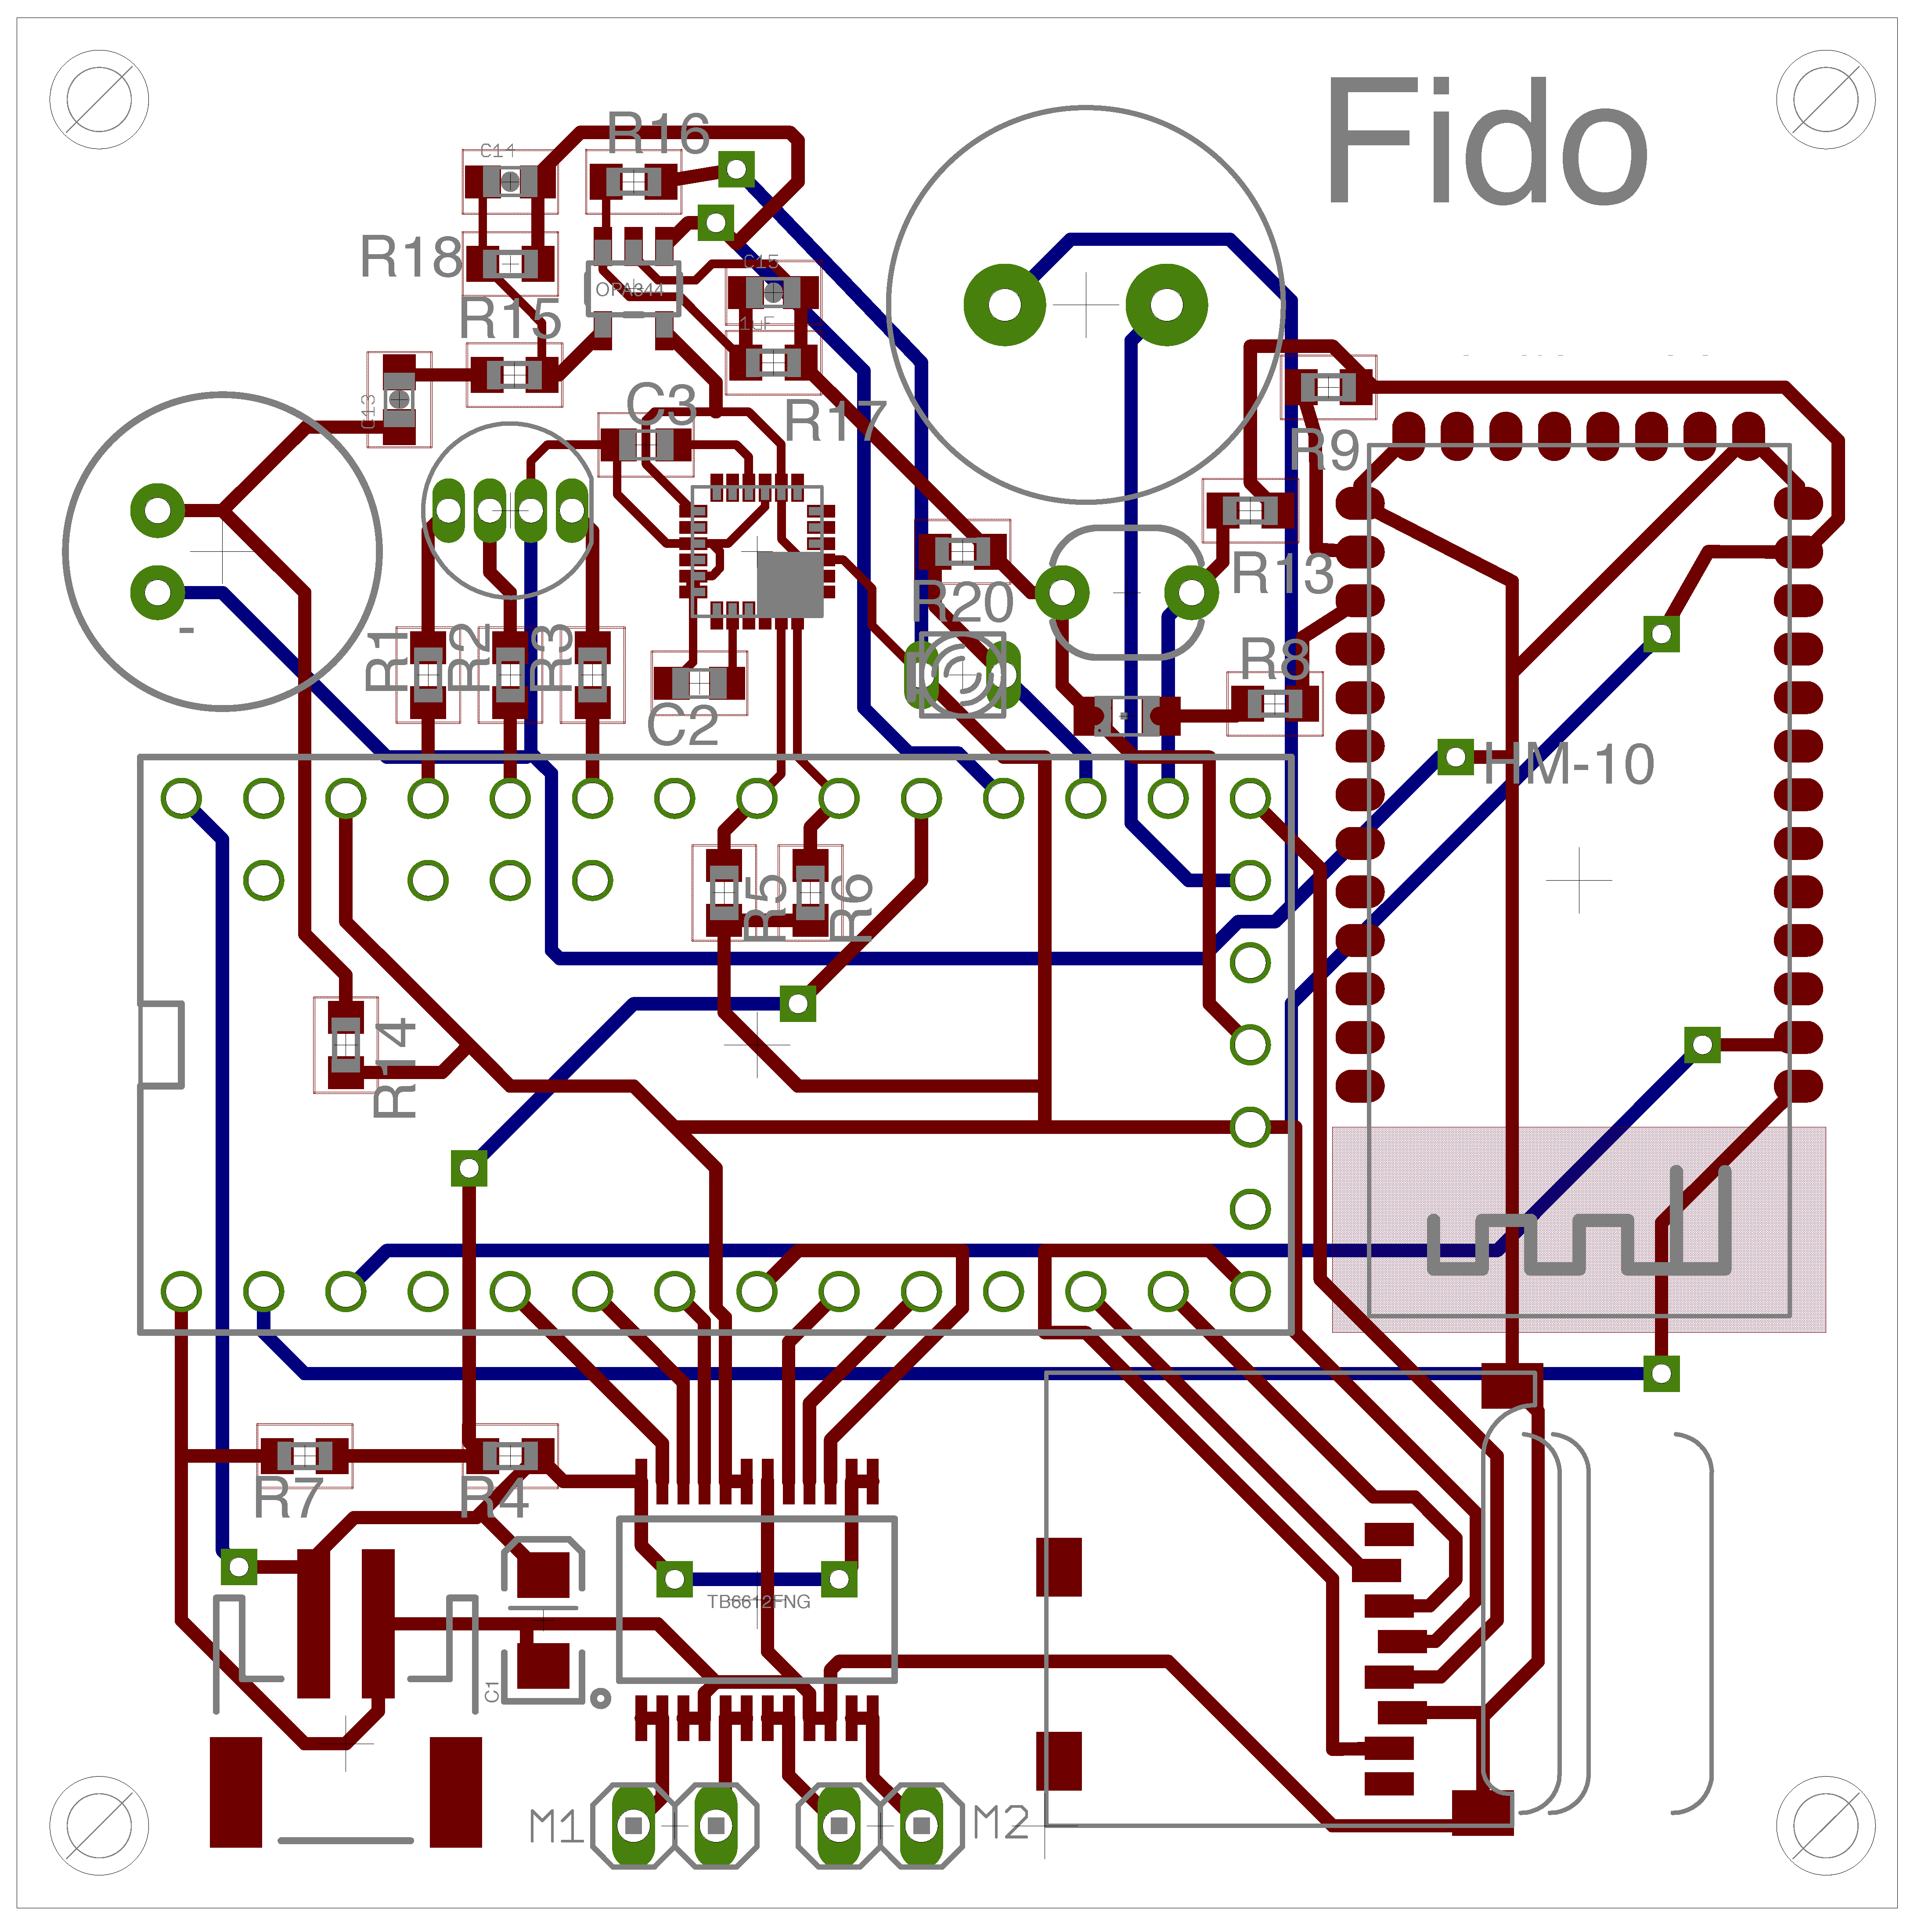
\includegraphics[height=7cm]{Figures/boardLayout.png}
	\caption{Fido PCB Layout}
\end{figure}

A schematic and printed circuit board have been designed for Fido's hardware implementation, and are the next step in testing and improving the Fido control system.  The PCB was modeled after the simulator reference design, and as such contains dual motor control, a photo-resistor for visible light, a photo-transistor for infrared light, etc.  The board (designed in CadSoft Eagle) operates off of the Teensy 3.1 microcontroller development platform, which combines a 96Mhz ARM Cortex M4 microcontroller and a USB bootloader for easy debugging.  The software base is in the process of being ported to the avr-gcc compiler toolchain for microcontrollers, a feat only possible through a small code footprint and low reliance on C++ Standard Library functionality.

\section{Conclusion}

A general robotic control system nicknamed Fido was developed that learned tasks with limited feed back. Fido couple the training of artificial neural networks with a wire-fitted moving least squares interpolator to achieve a continuous state-action space $Q$-learning reinforcement algorithm implementation. Fido leveraged a Boltzmann distribution of probability based on reward to select actions, allowing it to continuously explore its state-action space. A kinematically accurate robot was simulated with a differential drive system, a sensor array, and other outputs to test Fido. The robot was trained on a number of common robotic tasks and successfully converged on these tasks in less reward iterations than all other actors tested, while maintaining impressively low latency. In the future, we hope to improve Fido's software further and are working toward the completion of Fido's hardware implementation.

\nocite{wirefit,qlearn,backprop,practical,tutorial,kinematics}

\pagebreak
\bibliography{Sections/bibliography}
\bibliographystyle{apacite}

\end{document}